\section{City Selection}
\label{sec:city-selection}

This section presents an explanation of the city selection process.

\subsection{Criteria}

We carefully selected among several candidate cities, using the following criteria:

\begin{itemize}
    \item A city the team is familiar with, so that we can better understand the practical implications of our work.
    \item A city with well-defined borders, so that we can easily define a realistic environment.
    \item A city with reasonable complexity, not too big and not too small.
\end{itemize}

\subsection{Candidate Cities}

\begin{figure}
    \centering
    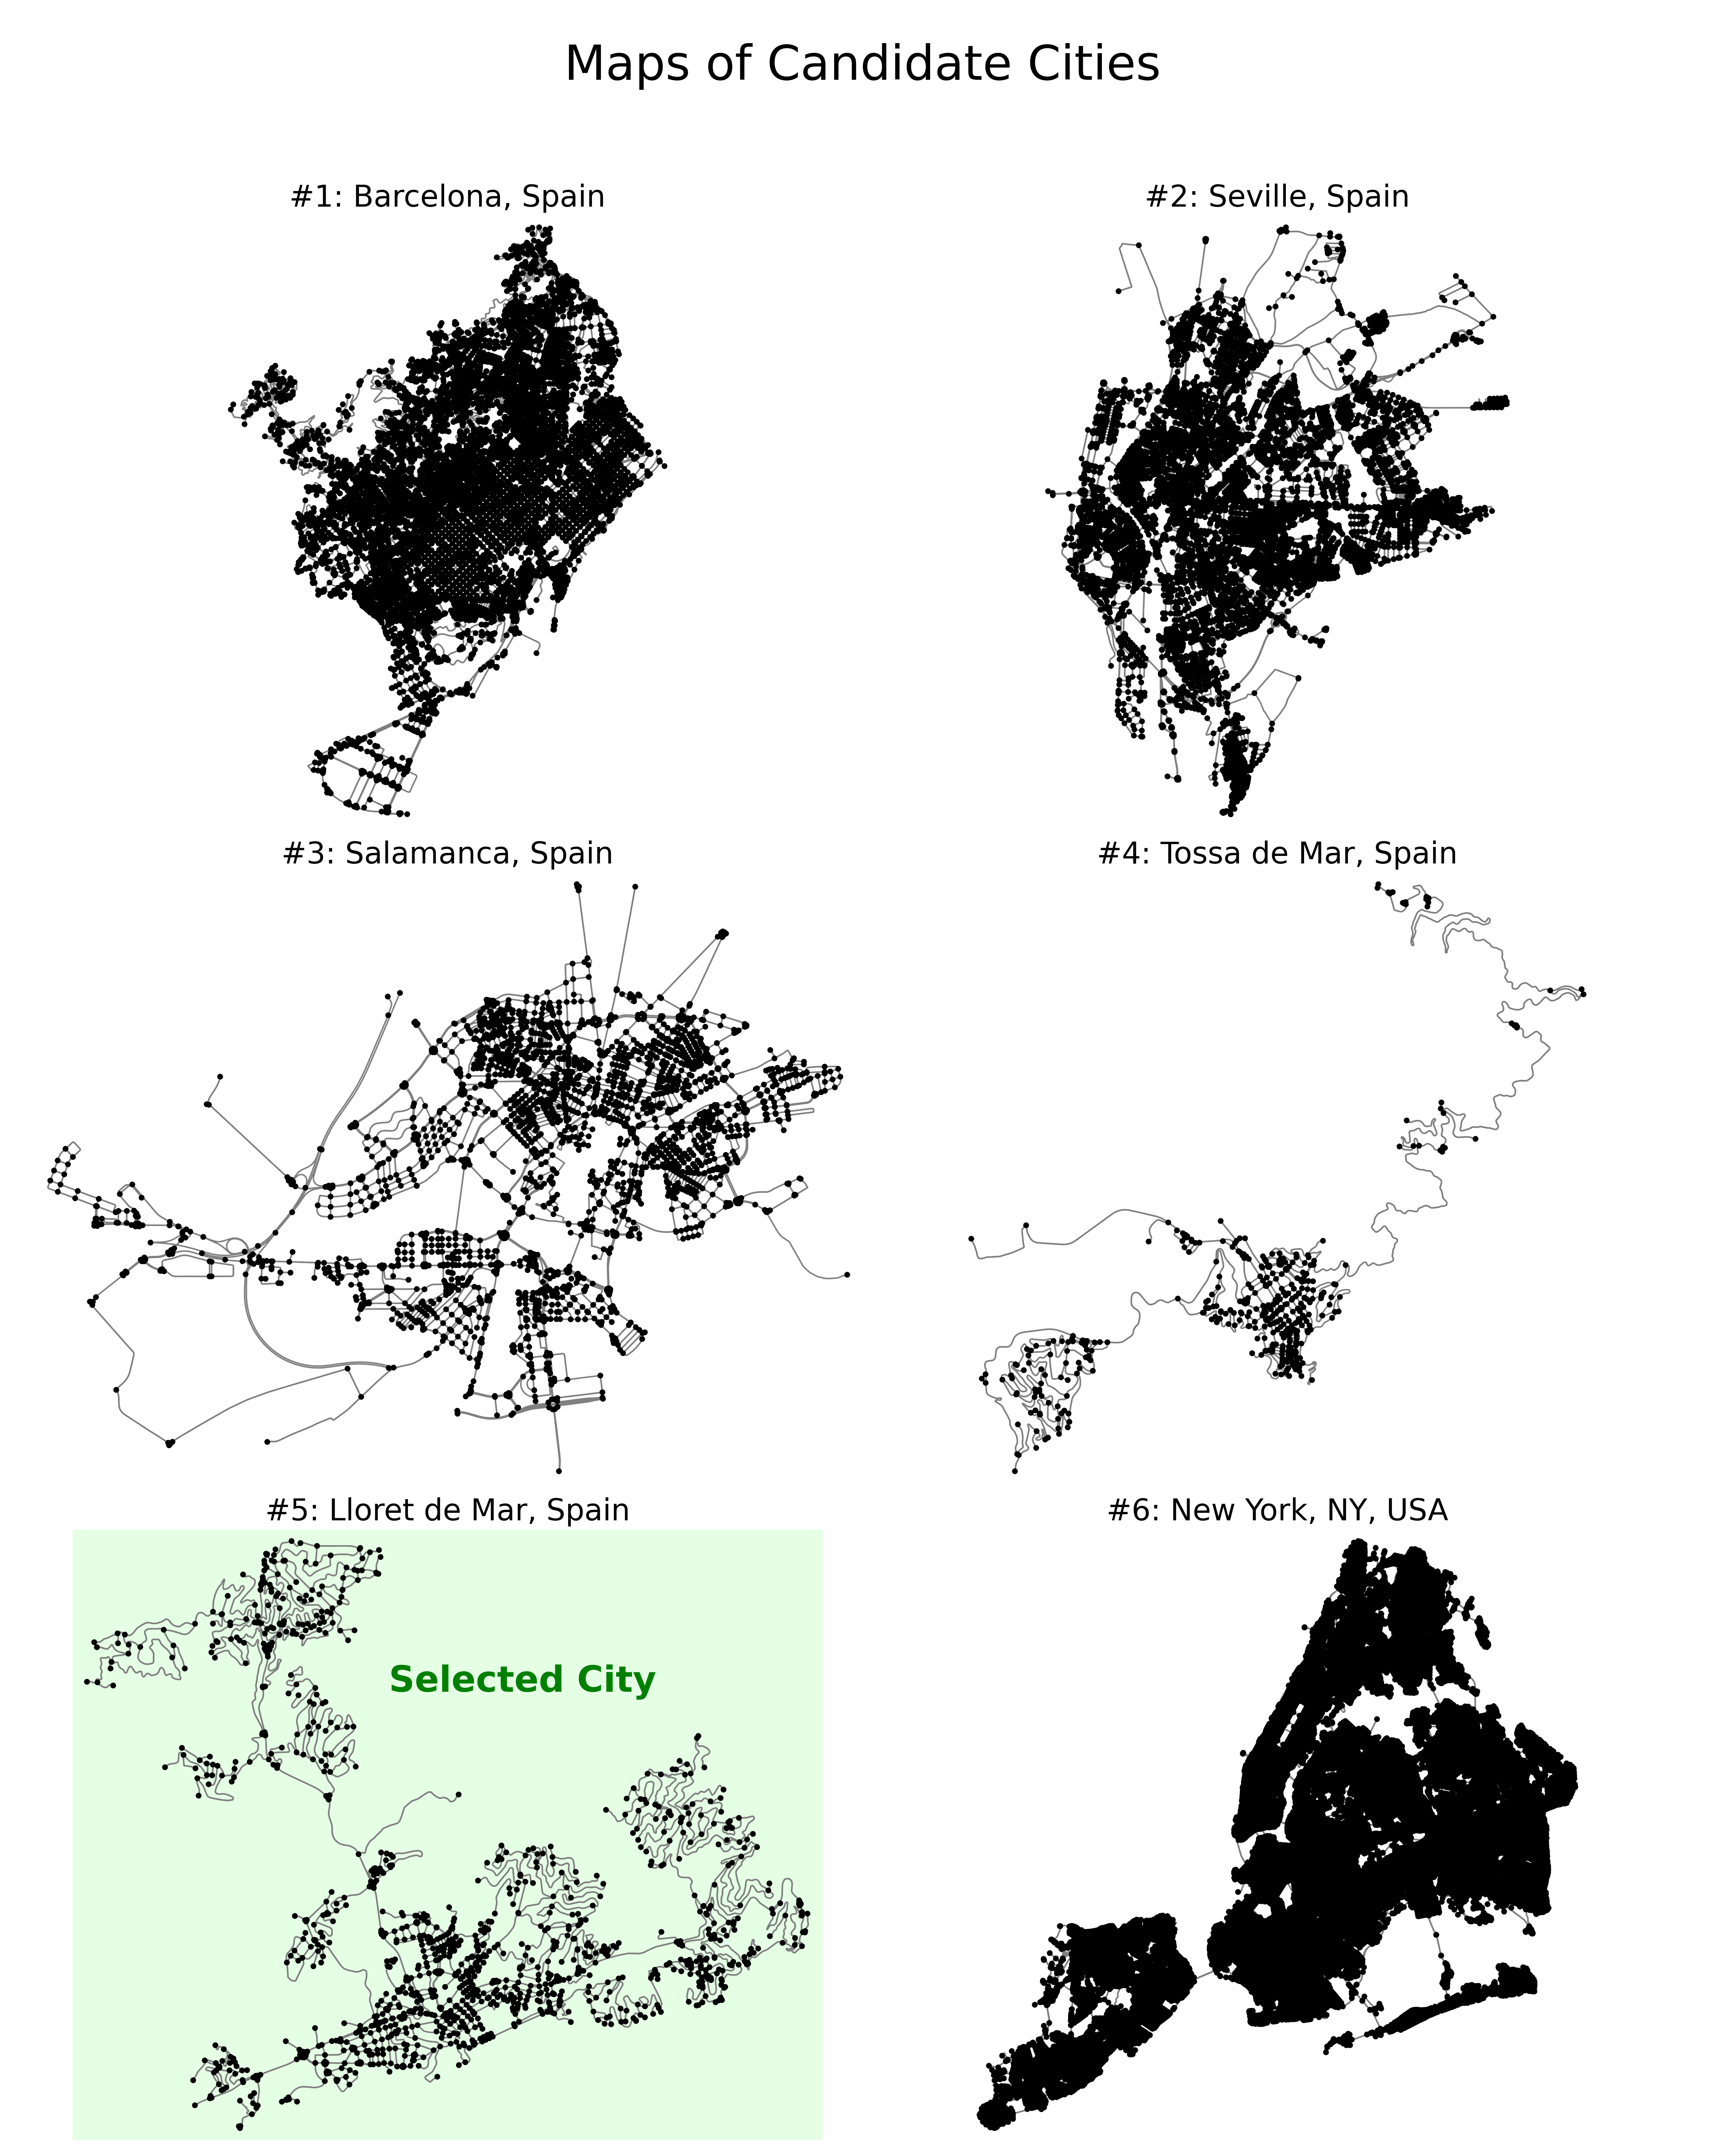
\includegraphics[width=0.8\textwidth]{../figures/maps_of_candidate_cities.png}
    \caption{Maps of Candidate Cities}
    \label{fig:candidate-cities}
\end{figure}

